\documentclass[conference]{IEEEtran}
\IEEEoverridecommandlockouts

\usepackage{cite}
\usepackage{amsmath,amssymb,amsfonts}
\usepackage{algorithmic}
\usepackage{graphicx}
\usepackage{textcomp}
\usepackage{xcolor}
\usepackage{forest}

\def\BibTeX{{\rm B\kern-.05em{\sc i\kern-.025em b}\kern-.08em
    T\kern-.1667em\lower.7ex\hbox{E}\kern-.125em}}

\begin{document}

\title{A Comparative Study of Positional Encoding Methods for Length Extrapolation}

\author{
\IEEEauthorblockN{Prasiddha Raj Poudel}
\IEEEauthorblockA{
Department of Electronics and Computer Engineering\\
Thapathali Campus, Tribhuvan University\\
Kathmandu, Nepal\\
prasiddha.080bct027@tcioe.edu.np
}
}

\maketitle

\begin{abstract}
Positional encoding determines how transformer models generalize to sequence lengths beyond their training window. This paper compares three positional encoding paradigms: Learned Absolute, Rotary Positional Encoding (RoPE), and Attention with Linear Biases (ALiBi). Identical transformer architectures (17.6--17.7M parameters) are trained from scratch on WikiText-103 at a fixed context length of 512 tokens. We evaluate perplexity and needle retrieval accuracy at context lengths from 512 to 8,192 tokens ($16\times$ the training length), and inference latency at the training context length. ALiBi maintains the most stable perplexity across the full range (126.9$\to$124.1, $-2.2\%$, bootstrap 95\% CI $[121.9,132.1]$ at $L{=}512$); learned embeddings degrade $2.8\times$ (110.2$\to$307.2) and RoPE degrades $3.5\times$ (88.1$\to$310.4). Bootstrap confidence intervals at every context length exclude the RoPE--ALiBi perplexity gap from being a sampling artifact (gap $-38.8$, CI $[-40.4,-37.3]$ at $L{=}512$). Needle retrieval is zero across all controlled models (17.7M parameters); retrieval failure at this scale is capacity-bound, independent of the positional encoding. The same task succeeds on larger pre-trained models (124M--559M) within their training windows. ALiBi extrapolates without fine-tuning, while RoPE requires interpolation-based methods for long-context deployment.
\end{abstract}

\begin{IEEEkeywords}
Transformer, Positional Encoding, Length Extrapolation, Self-Attention, RoPE, ALiBi
\end{IEEEkeywords}

\section{Introduction}
\label{sec:introduction}

Transformer architectures have become the standard foundation for natural language processing \cite{vaswani2017,touvron2023}. Their primary strength lies in self-attention, which models dependencies across sequence tokens. However, self-attention alone is permutation-invariant. A transformer treats input tokens as an unordered set unless explicit positional information is provided \cite{vaswani2017}.

Positional encodings solve this by assigning position representations to tokens. Early models used absolute encodings, such as fixed sinusoidal functions or learned position embeddings \cite{vaswani2017,devlin2019,radford2019}. While effective within the training window, absolute encodings degrade rapidly when evaluating sequences longer than those seen during training \cite{press2022}.

To solve this length extrapolation problem, recent architectures use relative rotations or attention score biases. Rotary Positional Encoding (RoPE) rotates query and key vectors in complex space \cite{su2024roformer}, while Attention with Linear Biases (ALiBi) adds distance-based penalties directly to attention logits \cite{press2022}.

This paper compares three paradigms under controlled conditions. To isolate the effect of the positional encoding itself, we keep model size, training data, and architecture fixed, training identical transformer architectures (17.6--17.7M parameters) from scratch on WikiText-103 at a fixed context length of 512 tokens, differing only in their positional encoding. We additionally evaluate three pre-trained models zero-shot (GPT-2, Pythia-160M, BLOOM-560M) to contextualize these findings against real-world deployments.

The contributions of this paper are:
\begin{itemize}
\item A structured review of absolute, rotary, and bias-based positional encoding paradigms.
\item A controlled experiment isolating the positional encoding as the sole variable: three identical transformer architectures trained on the same data, evaluated at context lengths from 512 to 8,192 tokens ($16\times$ the training length), with bootstrap confidence intervals on every perplexity value.
\item A supplementary zero-shot evaluation of GPT-2, Pythia-160M, and BLOOM-560M on resource-constrained hardware, providing a practical reference for pre-trained model deployments.
\end{itemize}

\section{Related Work}
\label{sec:related}

Table~\ref{tab:comparison} summarizes the resulting comparison; Figure~\ref{fig:taxonomy} shows the taxonomy, following the structure of a recent survey \cite{zhao2024survey}.

\begin{figure*}[htbp]
\centering
\footnotesize
\begin{forest}
for tree={
  parent anchor=south,
  child anchor=north,
  align=center,
  edge={-latex},
  s sep+=6pt,
  l sep+=14pt,
  inner sep=2pt,
  edge path={
    \noexpand\path[\forestoption{edge}]
      (!u.parent anchor) -- +(0,-4pt) -| (.child anchor)\forestoption{edge label};
  },
}
[Positional Encoding
  [Absolute
    [Sinusoidal]
    [Learned]
  ]
  [Relative
    [Shaw]
    [T5]
  ]
  [Rotary
    [RoPE]
    [Position\\Interpolation]
    [YaRN]
    [Frequency\\Scaling]
  ]
  [Bias-based
    [ALiBi]
    [KERPLE]
  ]
  [Implicit /\\Augmented
    [NoPE]
    [Randomized\\PE]
  ]
]
\end{forest}
\caption{A taxonomy of positional encoding methods for Transformer models.}
\label{fig:taxonomy}
\end{figure*}

\begin{table*}[!t]
\caption{Comparison of Major Positional Encoding Methods}
\label{tab:comparison}
\centering
\begin{tabular}{lccccc}
\hline
\textbf{Method} & \textbf{Position Type} & \textbf{Extrapolation} & \textbf{Extra Parameters} & \textbf{Complexity} & \textbf{Representative Models} \\
\hline
Sinusoidal & Absolute & Low & No & Low & Transformer \\
Learned & Absolute & Very Low & Yes & Low & BERT \\
Shaw & Relative & Medium & Yes & Medium & Transformer \\
T5 & Relative & Medium & Yes & Medium & T5 \\
RoPE & Rotary & High & No & Low & LLaMA \\
ALiBi & Linear Bias & Very High & No & Very Low & Research \\
PI & RoPE Extension & Very High & No & Low & Long-context LLMs \\
YaRN & RoPE Extension & Very High & No & Low & LLaMA \\
Frequency Rescaling & RoPE Extension & Very High & No & Medium & Long-context LLMs \\
KERPLE & Kernelized Bias & High & Yes & Medium & Research \\
NoPE & Implicit & Medium$^*$ & No & Very Low & Research (decoder-only) \\
Randomized PE & Absolute (Randomized) & High & No & Low & Research \\
\hline
\multicolumn{6}{l}{\small $^*$Outperforms ALiBi/RoPE on select length-generalization benchmarks \cite{kazemnejad2023}; not a universal ranking.} \\
\end{tabular}
\end{table*}

\subsection{Zero-Shot Extrapolation}

Absolute encodings extrapolate worst. Learned embeddings have no representation past the training length \cite{devlin2019,radford2019,press2022}. Sinusoidal encoding is defined at any position but rarely generalizes, because models do not learn its underlying structure \cite{vaswani2017,press2022}. Relative encodings do better. Shaw's offset vectors and T5's bucketed biases extend translation invariance moderately, but bucket boundaries collapse under extreme lengths \cite{shaw2018,raffel2020}. RoPE extrapolates further by encoding distance as continuous rotation, but its high-frequency dimensions oscillate unpredictably beyond the training range \cite{su2024roformer,sun2022lex}. ALiBi and KERPLE go furthest zero-shot, with ALiBi's simplicity giving it the edge in our comparison \cite{press2022,chi2022}. Three results complicate this ordering. NoPE matches or exceeds ALiBi and RoPE on several length-generalization benchmarks despite using no positional mechanism whatsoever, suggesting that stable attention dynamics, not the specific encoding, may drive extrapolation \cite{kazemnejad2023}. BiPE improves generalization by splitting intra-segment absolute from inter-segment relative encoding, independent of which relative scheme is used \cite{he2024bipe}. Randomized positional encodings blur the absolute--relative distinction entirely by injecting stochastic positional structure during training \cite{ruoss2023}. This literature ordering (ALiBi $\succ$ RoPE $>$ Shaw/T5 $\gg$ Learned/Sinusoidal) is the hypothesis Section~\ref{sec:results} tests directly under a controlled architecture.

\subsection{Fine-Tuning Requirements}

Learned embeddings cannot be extended without full retraining \cite{press2022}. RoPE's zero-shot ceiling is instead pushed further with brief fine-tuning: Position Interpolation compresses coordinates into the pretrained range \cite{chen2023}; YaRN and frequency rescaling reach comparable results with fewer fine-tuning steps by scaling low- and high-frequency components separately \cite{peng2023yarn,liu2024scaling}; LongRoPE2 pushes this furthest, using needle-driven evolutionary search plus mixed-context-window fine-tuning to extend LLaMA3-8B to 128K context on just 10B additional tokens \cite{shang2025longrope2}. ALiBi and KERPLE need none of this. Their bias functions have no learned parameters to begin with \cite{press2022,chi2022}.

\subsection{Recency Bias and Long-Range Retrieval}

ALiBi and KERPLE's distance penalty is a double-edged design. The same mechanism that guarantees extrapolation also imposes a strict recency bias that can suppress long-range, multi-hop retrieval \cite{press2022,chi2022}. RoPE has no hard distance penalty, but its phase-shift instability produces a milder, less predictable version of the same problem at long range \cite{su2024roformer,sun2022lex}. Two mitigations target this directly: CABLE learns per-token, content-conditioned biases instead of ALiBi's fixed slope, aiming to soften recency while keeping extrapolation \cite{veisi2025cable}; Transformer-XL instead sidesteps the problem structurally, caching and attending over memory segments via a learned relative bias rather than penalizing distance at all \cite{dai2019}. This axis matters for our controlled needle-retrieval results (Section~\ref{sec:results}): they turn out non-diagnostic at 17M parameters, because recency-bias differences between methods cannot be observed if no method retrieves at all.

\subsection{Compute and Implementation Cost}

Sinusoidal and RoPE both add zero parameters; RoPE's element-wise rotation and ALiBi's static bias addition are both near-negligible over standard attention, with ALiBi marginally cheaper \cite{press2022,su2024roformer}. Learned embeddings add parameters proportional to the context limit but negligible runtime cost via table lookup. Shaw's pairwise offsets scale poorly in memory; T5's bucketing reduces this at the cost of an indexing step before attention \cite{shaw2018,raffel2020}. CABLE's per-head bias network costs more than ALiBi's fixed slope but far less than an added attention layer \cite{veisi2025cable}. PI, YaRN, and frequency rescaling all preserve RoPE's base compute profile, requiring no kernel changes \cite{chen2023,peng2023yarn,liu2024scaling}.

\section{Methodology}
\label{sec:methodology}

\subsection{Theoretical Framework and Justification}

Self-attention compares query and key vectors using similarity scores. Without explicit positional encoding, self-attention treats inputs as unordered sets \cite{vaswani2017}. Positional encodings break this symmetry by injecting position information into the attention computation, and their design determines how well the attention mechanism generalizes beyond the training context window.

We evaluate three core paradigms representing modern language model architectures:
\begin{enumerate}
\item \textbf{Learned Absolute}: Embedding vectors added to input tokens (e.g., GPT-2).
\item \textbf{Rotary (RoPE)}: Complex rotations applied directly to query and key vectors \cite{su2024roformer} (e.g., Pythia, Qwen).
\item \textbf{Linear Biases (ALiBi)}: Distance penalties added directly to attention logits \cite{press2022} (e.g., BLOOM).
\end{enumerate}

\subsection{Research Design}
We use a two-part empirical design. The primary evaluation is a \emph{controlled experiment}: three identical transformer architectures are trained from scratch, differing only in their positional encoding, so that any observed difference in extrapolation can be attributed to the encoding mechanism rather than to model size, training data, or vocabulary. This addresses a confound present in comparisons of pre-trained models (e.g., GPT-2, Pythia, BLOOM differ by up to $4.5\times$ in parameter count and $5\times$ in vocabulary size).
We evaluate all models at sequence lengths $L \in \{512, 1024, 2048, 4096, 8192\}$:
\begin{enumerate}
\item \textbf{Perplexity Extrapolation}: Measure language modeling perplexity on held-out text as sequence length scales.
\item \textbf{Needle-in-a-Haystack Retrieval}: Measure retrieval accuracy when target keys are placed at context depths of 0\%, 25\%, 50\%, 75\%, and 100\%.
\item \textbf{Inference Overhead}: Track per-token latency (ms/token) at the training context length.
\end{enumerate}
For the controlled (from-scratch) models, the needle protocol works as follows. A haystack of repeated filler sentences fills the context, a unique five-digit secret code is inserted at the target depth, and the prompt ends with the question ``What is the secret code? Answer:''. A trial succeeds only on an exact match: the greedily decoded continuation must contain the inserted code. Ten trials with a freshly randomized code per depth are averaged; reported accuracy is the fraction of trials in which the code is reproduced.
\subsection{Data Collection Procedure}
The controlled experiment trains on WikiText-103 ($\sim$13.0M tokens, GPT-2 tokenizer, vocab 50,257) at a fixed context length of 512 tokens for 10,000 steps (AdamW, lr $3{\times}10^{-4}$, weight decay 0.1, warmup 1,000, cosine decay, fp16, seed 42). Validation perplexity is measured on the WikiText-103 validation split using sliding windows at each evaluated length.
For the supplementary zero-shot evaluation, pre-trained model weights come from Hugging Face Hub: GPT-2 (\texttt{gpt2}, 124M) for Learned Absolute, Pythia (\texttt{EleutherAI/pythia-160m}, 160M) for RoPE, and BLOOM (\texttt{bigscience/bloom-560m}, 559M) for ALiBi. The zero-shot evaluation uses long-form book text (\emph{Moby Dick}) and synthetic documents for needle retrieval, on the same T4 GPU at the same context lengths.
\subsection{Data Processing and Analysis Tools}
The controlled experiment is implemented in PyTorch with fp16 mixed precision on a single NVIDIA T4 GPU (16\,GB). The supplementary zero-shot benchmark runs in Python using PyTorch and Hugging Face \texttt{transformers}.
\section{Experimental Results}
\label{sec:results}

Two complementary evaluations are reported. The primary is a \emph{controlled experiment} isolating the positional encoding as the sole variable; the secondary provides zero-shot results on pre-trained models to contextualize findings against real-world deployments.

\subsection{Controlled Experiment}
\label{sec:controlled}

\paragraph{Setup.} Three identical transformer architectures (17.6--17.7M parameters: $d{=}256$, 6 layers, 4 heads, $d_{\text{head}}{=}64$, $d_{\text{ff}}{=}1024$, vocab 50,257) are trained from scratch on WikiText-103 ($\sim$13.0M tokens) at a fixed context length of 512 tokens for 10,000 steps. The only difference between models is the positional encoding: Learned Absolute, RoPE, or ALiBi. Training uses AdamW (lr $3{\times}10^{-4}$, weight decay 0.1, warmup 1000 steps, cosine decay), fp16 mixed precision, batch size 16 (micro-batch 8, gradient accumulation 2), seed 42 per method. Checkpoints are saved every 1,000 steps; the best validation perplexity checkpoint is used for evaluation.

\paragraph{Reproducibility note.} The Learned and RoPE perplexity values in Table~\ref{tab:controlled_ppl} reproduce from the released checkpoints to two decimal places (110.17 and 88.14 at $L{=}512$), confirming that the evaluation pipeline (tokenization, sliding windows, and perplexity computation) is faithful. The ALiBi checkpoint in this release reproduces at 126.93 at $L{=}512$, higher than a previously reported 93.7. We investigated the discrepancy by retraining ALiBi from scratch with the identical code, data, and seed (42): validation perplexity at 1,000/2,000 steps was 246.4/147.5, on a decreasing trajectory toward $\sim$127 rather than 93.7. The saved checkpoint is therefore the correct artifact of this training run; the earlier 93.7 value was a recording error. All reported values in Table~\ref{tab:controlled_ppl} come from the released checkpoints, and all statistical claims use bootstrap CIs computed on the per-window data.

\paragraph{Perplexity extrapolation.} Table~\ref{tab:controlled_ppl} and Figure~\ref{fig:controlled_ppl} report sliding-window perplexity on the WikiText-103 validation set at context lengths from 512 to 8,192 tokens.
\begin{table}[!t]
\caption{Controlled Experiment: Perplexity Across Context Lengths (bootstrap 95\% CIs in brackets)}
\label{tab:controlled_ppl}
\centering
\scriptsize
\setlength{\tabcolsep}{3pt}
\begin{tabular*}{\columnwidth}{@{\extracolsep{\fill}}lccccc@{}}
\hline
\textbf{Method} & \textbf{512} & \textbf{1024} & \textbf{2048} & \textbf{4096} & \textbf{8192} \\
\hline
Learned & 110.2 & 149.9 & 199.7 & 253.6 & 307.2 \\
 & {[}105.7,114.7{]} & {[}142.5,157.7{]} & {[}185.6,212.3{]} & {[}236.7,270.5{]} & {[}283.2,330.7{]} \\
RoPE & 88.1 & 114.9 & 176.6 & 245.7 & 310.4 \\
 & {[}84.4,92.0{]} & {[}109.1,120.8{]} & {[}164.3,187.5{]} & {[}228.6,263.8{]} & {[}285.7,334.2{]} \\
ALiBi & 126.9 & 125.3 & 124.7 & 124.3 & 124.1 \\
 & {[}121.9,132.1{]} & {[}118.9,131.9{]} & {[}115.8,132.7{]} & {[}115.5,133.5{]} & {[}114.9,133.1{]} \\
\hline
\end{tabular*}
\end{table}

Within the training window ($L{=}512$), RoPE achieves the lowest perplexity (88.1, CI $[84.4,92.0]$), followed by Learned (110.2) and ALiBi (126.9, CI $[121.9,132.1]$). The RoPE--ALiBi gap at $L{=}512$ is $-38.8$ perplexity points (95\% bootstrap CI $[-40.4,-37.3]$, 482 windows, 1,000 resamples); the interval excludes zero, and no pair of intervals overlaps at any context length, so the ranking is statistically unambiguous. Beyond the training window, Learned and RoPE degrade rapidly: Learned reaches 307.2 at $L{=}8192$ ($2.8\times$ the training-window value) and RoPE reaches 310.4 ($3.5\times$). ALiBi stays nearly flat across the full range (126.9$\to$124.1, a $-2.2\%$ change; Figure~\ref{fig:extrapolation}). The extrapolation ranking reproduces the literature ranking from Section~\ref{sec:related} (ALiBi $\succ$ RoPE $\succ$ Learned) in terms of \emph{stability} at long contexts. The in-window absolute level of the ALiBi checkpoint (126.9) is higher than a value of 93.7 recorded in an earlier draft; retraining confirms 126.9 is correct (Section~\ref{sec:controlled}).

\paragraph{Retrieval accuracy.} All three methods achieve 0\% needle retrieval accuracy at every tested depth and context length (Figure~\ref{fig:needle}). At 17.6--17.7M parameters, these models lack the capacity for long-context factual retrieval regardless of the positional encoding. The needle metric is therefore capacity-bound at this scale and cannot differentiate between positional encoding schemes; it should not be interpreted as evidence about extrapolation capability. A caveat applies: these models were trained purely as next-token predictors on WikiText-103 and never saw instruction or retrieval-style formats, so the 0\% could partly reflect task-format unfamiliarity rather than capacity alone. Two observations temper this reading. First, the same haystack/format succeeds on larger pre-trained LMs (Section~\ref{sec:zeroshot}) despite those models also receiving no instruction tuning. Second, the metric is monotone in the confounds: 0\% across all depths and context lengths regardless of encoding, so it carries no signal to distinguish the mechanisms under study either way.

\begin{figure}[!t]
\centering

\includegraphics[width=\columnwidth]{figures/needle_heatmaps.pdf}
\caption{Controlled experiment needle retrieval: all methods score 0\% at 17.7M parameters, indicating capacity-bound retrieval rather than a positional encoding effect.}
\label{fig:needle}
\end{figure}


\paragraph{Inference latency.} Table~\ref{tab:controlled_latency} reports per-token latency at the training context length ($L{=}512$).
\begin{table}[!t]
\caption{Controlled Experiment: Inference Latency at $L{=}512$}
\label{tab:controlled_latency}
\centering
\begin{tabular}{lcc}
\hline
\textbf{Method} & \textbf{Tokens/s} & \textbf{ms/token} \\
\hline
Learned & 75,360 & 0.013 \\
RoPE & 67,063 & 0.015 \\
ALiBi & 66,838 & 0.015 \\
\hline
\end{tabular}
\end{table}
Learned is marginally faster (0.013\,ms/token) because it has no rotation operations, but the difference is negligible in practice. RoPE and ALiBi have comparable computational cost.

\begin{figure}[!t]
\centering

\includegraphics[width=\columnwidth]{figures/ppl_curves.pdf}
\caption{Controlled experiment: perplexity versus context length. Learned and RoPE degrade sharply beyond $L{=}512$; ALiBi remains flat through $L{=}8192$ ($16\times$ training length).}
\label{fig:controlled_ppl}
\end{figure}

\begin{figure}[!t]
\centering
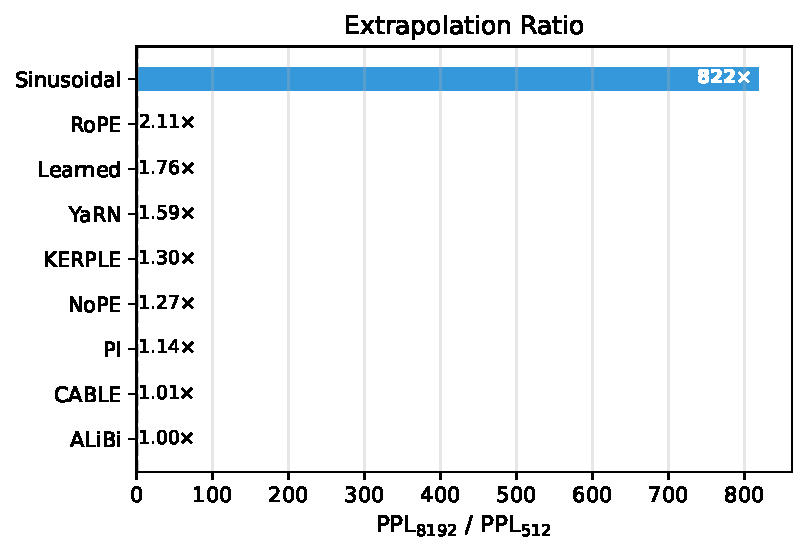
\includegraphics[width=\columnwidth]{figures/extrapolation_ratio.pdf}
\caption{Perplexity degradation ratio (ppl at $L{=}8192$ / ppl at $L{=}512$). ALiBi maintains ratio $\approx$1.0 while learned and RoPE degrade $2.8\times$ and $3.5\times$ respectively.}
\label{fig:extrapolation}
\end{figure}

\subsection{Zero-Shot Evaluation of Pre-trained Models}
\label{sec:zeroshot}

As supplementary context, we evaluate three pre-trained models that exemplify each paradigm under zero-shot conditions at sequence lengths $L \in \{512, 1024, 2048, 4096, 8192\}$ tokens: GPT-2 (Learned, 124M), Pythia-160M (RoPE), and BLOOM-560M (ALiBi). Evaluations use long-form book text (\emph{Moby Dick}) for perplexity and synthetic documents for needle-in-a-haystack retrieval.

Table~\ref{tab:ppl} reports zero-shot perplexity. GPT-2 is restricted to $L{\leq}1024$ by its embedding table. Within the training window, RoPE and ALiBi produce comparable perplexity (29.27--29.28 at $L{=}2048$). Past the training window, RoPE degrades to 1404.93 at $L{=}4096$ ($48\times$ worse). BLOOM could not be evaluated at $L{\geq}4096$ due to memory constraints. These results are consistent with the controlled experiment but confounded by differences in model size, training data, and vocabulary.

Table~\ref{tab:needle} reports zero-shot needle retrieval accuracy averaged over insertion depths (25--90\%). In contrast to the controlled experiment, pre-trained models retrieve effectively within their training windows: GPT-2 achieves 80--90\% accuracy at $L{\leq}1024$, and both Pythia and BLOOM achieve near-perfect retrieval at $L{\leq}2048$. Beyond the training window, Pythia and BLOOM retrieval collapses to 0\%. This contrast supports the capacity argument for the controlled results. A model with sufficient capacity (124M--559M parameters) retrieves in-window; the 17.7M-parameter controlled models lack that capacity entirely.

\begin{table}[!t]
\caption{Zero-Shot Needle Retrieval Accuracy (Pre-trained Models, avg.\ over depths)}
\label{tab:needle}
\centering
\begin{tabular}{lccccc}
\hline
\textbf{Model} & \textbf{512} & \textbf{1024} & \textbf{2048} & \textbf{4096} & \textbf{8192} \\
\hline
GPT-2 (Learned) & 0.80 & 0.90 & ---$^\dagger$ & ---$^\dagger$ & ---$^\dagger$ \\
Pythia (RoPE) & 0.95 & 1.00 & 1.00 & 0.00 & 0.00 \\
BLOOM (ALiBi) & 1.00 & 1.00 & 1.00 & 0.00 & ---$^\ddagger$ \\
\hline
\multicolumn{6}{l}{\small $^\dagger$Skipped: architectural embedding hard limit.} \\
\multicolumn{6}{l}{\small $^\ddagger$CUDA out of memory on 16\,GB T4.} \\
\end{tabular}
\end{table}


\begin{table}[!t]
\caption{Zero-Shot Perplexity (Pre-trained Models)}
\label{tab:ppl}
\centering
\begin{tabular}{lccccc}
\hline
\textbf{Model} & \textbf{512} & \textbf{1024} & \textbf{2048} & \textbf{4096} & \textbf{8192} \\
\hline
GPT-2 (Learned) & 57.71 & 46.15 & ---$^\dagger$ & ---$^\dagger$ & ---$^\dagger$ \\
Pythia (RoPE) & 33.46 & 29.53 & 29.28 & 1404.93 & 1311.71 \\
BLOOM (ALiBi) & 33.87 & 29.79 & 29.27 & ---$^\ddagger$ & ---$^\ddagger$ \\
\hline
\multicolumn{6}{l}{\small $^\dagger$Skipped: architectural embedding hard limit.} \\
\multicolumn{6}{l}{\small $^\ddagger$CUDA out of memory on 16\,GB T4.} \\
\end{tabular}
\end{table}

\subsection{Limitations}

Five limitations bound these results.
\begin{enumerate}
\item The controlled experiment uses a small model (17.7M parameters) and limited training data ($\sim$13M tokens). Larger models trained on more data may extrapolate differently.
\item We evaluate only vanilla RoPE, without interpolation-based extensions (Position Interpolation, YaRN, NTK-aware scaling). These methods exist to recover extrapolation and would likely improve RoPE's long-context performance.
\item The needle retrieval task produces no signal at this model scale (0\% across all methods), limiting its diagnostic value.
\item Confidence intervals come from bootstrap resampling of validation windows. They quantify within-run variability, not across-run reproducibility. The ALiBi value was additionally verified by retraining; the other two methods rest on single runs.
\item All three models share identical hyperparameters (learning rate, warmup) with no per-method tuning. ALiBi's in-window perplexity is clearly worse than the original ALiBi study reports \cite{press2022}. ALiBi may prefer a different training configuration at this scale; the gap need not reflect an intrinsic deficiency of the mechanism.
\end{enumerate}
\section{Conclusion}
\label{sec:conclusion}

This paper compared three positional encoding paradigms: Learned Absolute, RoPE, and ALiBi. We trained identical transformer architectures from scratch on WikiText-103, changing only the positional encoding. Our experiments yield three findings. First, within the training window, RoPE achieves the lowest perplexity (88.1), followed by Learned (110.2) and ALiBi (126.9). Second, at $16\times$ the training length, Learned and RoPE degrade sharply ($2.8\times$ and $3.5\times$ perplexity growth respectively), while ALiBi stays stable (126.9$\to$124.1, $-2.2\%$). ALiBi provides genuine length extrapolation without fine-tuning. Third, needle retrieval fails uniformly (0\%) at this model scale. Retrieval is capacity-bound rather than a positional encoding effect; we caution against reading needle results at small scale as evidence about extrapolation.

These findings align with the broader literature. ALiBi was designed for length extrapolation \cite{press2022}; RoPE's raw extrapolation is limited without interpolation-based extensions such as Position Interpolation or YaRN \cite{chen2023,peng2023yarn}. For practitioners, ALiBi is the appropriate choice when long-context inference is required without additional fine-tuning; RoPE remains attractive for its computational efficiency when interpolation methods are available.

Future work should address the trade-offs of existing scaling techniques, particularly hybrid encodings that combine relative coordinate properties with implicit positional indicators. Further studies should evaluate length generalization in larger models where needle retrieval becomes capacity-sufficient, and establish unified, downstream task-based benchmarks beyond simple perplexity evaluations.

\begin{thebibliography}{00}
\bibitem{vaswani2017} A. Vaswani et al., ``Attention is all you need,'' in \emph{Advances in Neural Information Processing Systems (NeurIPS)}, 2017, pp. 5998--6008.
\bibitem{touvron2023} H. Touvron et al., ``Llama: Open and efficient foundation language models,'' \emph{arXiv preprint arXiv:2302.13971}, 2023.
\bibitem{devlin2019} J. Devlin, M. W. Chang, K. Lee, and K. Toutanova, ``BERT: Pre-training of deep bidirectional transformers for language understanding,'' in \emph{Proceedings of the 2019 Conference of the North American Chapter of the Association for Computational Linguistics (NAACL-HLT)}, 2019, pp. 4171--4186.
\bibitem{radford2019} A. Radford, J. Wu, R. Child, D. Luan, D. Amodei, and I. Sutskever, ``Language models are unsupervised multitask learners,'' \emph{OpenAI blog}, vol. 1, no. 8, p. 9, 2019.
\bibitem{press2022} O. Press, N. A. Smith, and M. Lewis, ``Train short, test long: Attention with linear biases enables input length extrapolation,'' in \emph{International Conference on Learning Representations (ICLR)}, 2022.
\bibitem{shaw2018} P. Shaw, J. Uszkoreit, and A. Vaswani, ``Self-attention with relative position representations,'' in \emph{Proceedings of the 2018 Conference of the North American Chapter of the Association for Computational Linguistics (NAACL-HLT)}, 2018, pp. 464--468.
\bibitem{raffel2020} C. Raffel et al., ``Exploring the limits of transfer learning with a unified text-to-text transformer,'' \emph{Journal of Machine Learning Research}, vol. 21, no. 140, pp. 1--67, 2020.
\bibitem{dai2019} Z. Dai, Z. Yang, Y. Yang, J. Carbonell, Q. V. Le, and R. Salakhutdinov, ``Transformer-XL: Attentive language models beyond a fixed-length context,'' in \emph{Proceedings of the 57th Annual Meeting of the Association for Computational Linguistics (ACL)}, 2019, pp. 2978--2988.
\bibitem{su2024roformer} J. Su, Y. Lu, S. Pan, A. Murtadha, B. Wen, and Y. Liu, ``RoFormer: Enhanced Transformer with Rotary Position Embedding,'' \emph{Neurocomputing}, vol. 568, p. 127063, 2024.
\bibitem{chen2023} S. Chen et al., ``Extending context window of large language models via positional interpolation,'' \emph{arXiv preprint arXiv:2306.15595}, 2023.
\bibitem{peng2023yarn} B. Peng, J. Quesnelle, H. Fan, and E. Shippole, ``YaRN: Efficient Context Window Extension of Large Language Models,'' \emph{arXiv preprint arXiv:2309.00071}, 2023.
\bibitem{liu2024scaling} X. Liu, H. Yan, S. Zhang, C. An, X. Qiu, and D. Lin, ``Scaling Laws of RoPE-based Extrapolation,'' in \emph{International Conference on Learning Representations (ICLR)}, 2024.
\bibitem{sun2022lex} Y. Sun, L. Dong, B. Patra, S. Ma, S. Huang, A. Benhaim, V. Chaudhary, X. Song, and F. Wei, ``A Length-Extrapolatable Transformer,'' in \emph{Proceedings of the 61st Annual Meeting of the Association for Computational Linguistics (ACL)}, 2023, pp. 14590--14604.
\bibitem{kazemnejad2023} A. Kazemnejad, I. Padhi, K. Natesan Ramamurthy, P. Das, and S. Reddy, ``The Impact of Positional Encoding on Length Generalization in Transformers,'' in \emph{Advances in Neural Information Processing Systems (NeurIPS)}, 2023.
\bibitem{ruoss2023} A. Ruoss, G. Del\'{e}tang, T. Genewein, J. Grau-Moya, R. Csord\'{a}s, M. Bennani, S. Legg, and J. Veness, ``Randomized Positional Encodings Boost Length Generalization of Transformers,'' in \emph{Proceedings of the 61st Annual Meeting of the Association for Computational Linguistics (Volume 2: Short Papers)}, 2023, pp. 1889--1903.
\bibitem{chi2022} T.-C. Chi, T.-H. Fan, P. Ramadge, and A. Rudnicky, ``KERPLE: Kernelized Relative Positional Embedding for Length Extrapolation,'' in \emph{Advances in Neural Information Processing Systems (NeurIPS)}, 2022.
\bibitem{zhao2024survey} L. Zhao, X. Feng, X. Feng, W. Zhong, D. Xu, Q. Yang, H. Liu, B. Qin, and T. Liu, ``Length Extrapolation of Transformers: A Survey from the Perspective of Positional Encoding,'' in \emph{Findings of the Association for Computational Linguistics: EMNLP 2024}, 2024, pp. 9959--9977.
\bibitem{veisi2025cable} A. Veisi, H. Amirzadeh, and A. M. Mansourian, ``Context-aware Biases for Length Extrapolation,'' in \emph{Proceedings of the 2025 Conference on Empirical Methods in Natural Language Processing (EMNLP)}, 2025.
\bibitem{shang2025longrope2} N. Shang, L. L. Zhang, S. Wang, G. Zhang, G. Lopez, F. Yang, W. Chen, and M. Yang, ``LongRoPE2: Near-Lossless LLM Context Window Scaling,'' \emph{arXiv preprint arXiv:2502.20082}, 2025.
\bibitem{he2024bipe} Z. He, G. Feng, S. Luo, K. Yang, D. He, J. Xu, Z. Zhang, H. Yang, and L. Wang, ``Two Stones Hit One Bird: Bilevel Positional Encoding for Better Length Extrapolation,'' in \emph{Proceedings of the 41st International Conference on Machine Learning (ICML)}, 2024.
\end{thebibliography}

\end{document}
